%Chapter 1 - Intro

\section{History}
%BRIEF HISTORY

%Rutherford
Ernest Rutherford performed what is often considered the first scattering experiment. This experiment fired an $\alpha$-particle beam at gold foil. The result of this experiment saw most particles pass through the foil completely undeflected. Those that did deflect were scattered at a large range of angles. This gave the world a new view of the nucleus, that of a largely empty space with a few hard scattering centers. We now know that these scattering centers are the nucleus of the atom, formed by a dense combination of protons and neutrons.\cite{GRIF}

Since this time, many experiments have been conducted that expanded our view of the nucleus. The evidence of quarks at SLAC once again revolutionized our understanding of the nucleus. In this experiment, electrons were scattered off protons over a large momentum transfer, $q^2$, and final hadronic invariant mass, $W$, range. This experiment noted a ``surprisingly weak'' $q^2$ dependence once the kinematics reached the $W>2 \textrm{GeV}$ range, a key feature of Deep Inelastic Scattering.\cite{SLAC_DIS} In this view the nucleons, protons and neutrons, are comprised of quarks. These quarks are elementary particles that define the characteristics and structure of the nucleon.\cite{DoQ}

This discovery paved the way for a wave of Deep Inelastic Scattering experiments. These experiments have refined our understanding of the nucleus and its constituent components. Deep Inelastic Scattering has proven to be a one of the most powerful tools available when one seeks to study nuclear structure.

%8-fold way
%As more and more particles were discovered, physicists began looking for an underlying order. In 1961, Murray Gell-Mann and Yuval Ne'eman independently proposed a scheme to explain the abundance of hadrons called SU(3) symmetry. This method groups baryons into categories of spin. From there, using the strangeness and charge an organization scheme appears. 
%
%Gell-Mann designed a graphical representation of these symmetries, which he dubbed the \textit{Eightfold Way}. The spin-0 mesons and spin-\nicefrac{1}{2} octets are each drawn as a hexagon with two particles in the center. The spin-\nicefrac{3}{2} decuplet is drawn as an upside-down triangle. When this method was proposed, all particles in the spin-\nicefrac{3}{2} decuplet were discovered except for the bottom point. Lending credence to this explanation was the prediction, and subsequent discovery, of the $\Omega^-$ particle.
%\cite{DoQ}\cite{GRIF}
%
%%Gell-Mann and Zweig
%%The Quark-Parton Model describes the composition of hadrons, both baryons and mesons. Prior to 1964, it was believed that hadrons were as small as it got. However, the adherence of hadrons to the eight-fold way, a categorization of hadrons by charge and strangeness, suggested that there was some underlying mechanism that had yet to be discovered.
%
%The adherence of hadrons to SU(3) symmetry lacked explanation. In 1964, Gell-Mann and Zweig independently suggested that hadrons could be composed smaller elementary particles. Gell-Mann offered the name ``quarks'' for these constituents. Three quarks were described to be the fundamental building blocks of all known particles: up, down, and strange. These quarks (and their corresponding antiquarks) were purported to be mathematical constructs with fractional charge, \nicefrac{2}{3} for up and \nicefrac{1}{3} for down and strange.
%
%Furthering the theory, in November 1974 two separate experiments published the discovery of the (now named) $J/\psi$ particle. The long lifetime of the $J/\psi$ suggested that new physics must be at play. The Quark-Parton Model predicted the existence of a quark symmetric to the strange quark, called the charm quark. It was determined that the $J/\psi$ could be a meson comprised of a charm and anti-charm, suggesting the validity of the model.

\section{Electron Scattering}
Electron scattering allows for finely tuned analysis of the nucleus. By manipulating the energy of the incoming electron and the kinematic variables accepted by the detectors used, experimenters can choose what aspect of the nucleus will be probed. This technique has been used to study the structure of the nucleus all the way down to the properties of the constituent quarks.

There are four kinematic regimes of electron scattering that can be explored: elastic, quasi-elastic, resonance, and deep inelastic scattering. Each of these regimes are defined by the kinematics and the underlying physical structure that they are sensitive to.

Elastic scattering occurs when the electron scatters coherently off of the nucleus. This occurs at low momentum and energy transfer. At these kinematics, the electron is sensitive to the size of the nucleus. The size of the nucleus is accessed by extracting nuclear ``form factors'' from the measured cross sections. From this we can learn about the charge distributions, magnetic moments, and charge radius of the nucleus.

Quasi-elastic scattering occurs at larger energy transfers when the electron scatters elastically off of the nucleon, rather than the nucleus. At these kinematics, the electron is sensitive to the form factors of the nucleon.

Resonance scattering occurs at even larger momentum and energy transfers. In this region, some of the energy is used to excite the nucleon into a higher energy state, called a resonance. A resonance is a short-lived particle. The resonance will quickly decay back into the nucleon and emit the excess energy as an additional particle. For example, $ep \rightarrow e\Delta^+ \rightarrow ep\pi^0$.

As we push the momentum and energy transfer further, we enter the Deep Inelastic Scattering (DIS) region. As $Q^2$ is increased into the transition region between resonance and DIS, the resonance peaks begin to smooth out. Here the electron becomes sensitive to the constituent parts of the nucleon. The wavelength of the exchanged photon is inversely proportional to $Q^2$. DIS scattering is of particular interest because the wavelength is sufficiently small enough to discern the parton structure. Through careful measurement, we can access the nuclear structure functions and the parton distributions in the the nucleons \cite{HaM,PaN,NaPP}.

The MARATHON experiment seeks to study the nuclear and nucleon structure functions, as well as nucleon parton distributions. The kinematics used are in the DIS region in order to facilitate this study. The remainder of this chapter will be focused on the DIS cross section and what we can learn from it.

%Inelastic scattering allows us to probe the internal structure of the nucleon. As $Q^2$ increases, baryon resonances begin to appear. As we push $Q^2$ even further past the resonance region, the wavelength of the virtual photon exchanged is short enough to discern the quark structure. This is known as the Deep Inelastic Scattering region.

\subsection{Deep Inelastic Scattering Cross Section}

Deep Inelastic Scattering, shown in Figure \ref{fig:feyn_dis}, involves a high energy electron scattering off of a nucleon. In the lowest order perturbation, a virtual photon is exchanged between the electron and nucleon. This momentum transfer then excites the nucleon into a hadronic final state. Though the final hadronic state is undetected, the detection of the scattered electron can yield insight into the interaction.

The reaction for scattering off a proton, is written as:

\begin{equation*}
	e^- + P \rightarrow e^- + X
\end{equation*}

\begin{figure}
\begin{center}
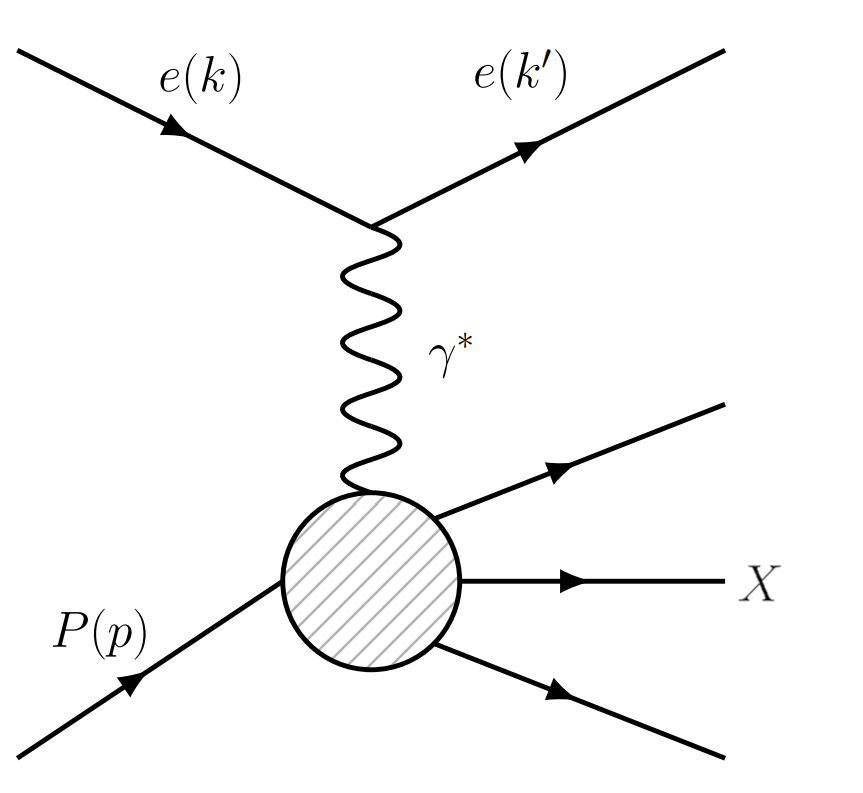
\includegraphics[width=.5\textwidth]{./scattering/fig/feyn_dis.png}
\caption{Feynman Diagram of Deep Inelastic Scattering}
\label{fig:feyn_dis}
\end{center}
\end{figure}

In this section, there will be many variables defined. For clarity, the meaning of these variables are defined in Table \ref{tab:var_def}. Mathematical definitions will follow, as necessary.

\begin{table}
\center
\begin{tabular}{|l|l|}
\hline 
$Q^2$ & Negative of the 4-momentum transfer \\
$W^2$ & Square of the invariant mass of the final hadronic state \\
$E$ & Beam energy \\
$E^\prime$ & Scattered electron energy \\
$L_{\mu\nu}$ & Electron tensor \\
$W^{\mu\nu}$ & Symmetric hadronic tensor \\
$k$ & 4-momentum of the incident electron \\
$k^\prime$ & 4-momentum of the scattered electron \\
$p$ & 4-momentum of the target nucleon \\
$\theta$ & Scattered electron angle \\
$\nu$ & Energy difference between incoming and scattered electron \\
$M$ & Proton mass \\
$m$ & Electron mass \\
\hline
\end{tabular}
\caption{Variable definitions introduced in this section}
\label{tab:var_def}
\end{table}

The kinematics of scattering are typically defined by the Lorentz-invariant kinematic variables $Q^2$ and $W^2$, as well as the energy difference $\nu$. These variables are defined as:

\begin{equation}
	q^2 \equiv -Q^2 = \left(k-k^\prime\right)^2
\end{equation}

\begin{equation}
	W^2 = \left(p+q\right)^2
\end{equation}

\begin{equation}
	\nu = E-E^\prime
\end{equation}

Now it is useful to analyze in the laboratory rest frame and to note that MARATHON is a fixed target experiment. In this frame, the target is ``at rest'' (i.e. having a four-momentum of $\left(M,0\right)$). This leads to a simplification of $Q^2$ and $W^2$.

\begin{equation}
	Q^2 = 4EE^\prime\sin^2\frac{\theta}{2}
\end{equation}

\begin{equation}
	W^2 = M^2 + 2M\nu - Q^2
\end{equation}

Electron-nucleon scattering can be generally expressed as the following:

\begin{equation}
	\frac{d^2\sigma}{d\Omega dE^\prime} = \frac{\alpha^2}{Q^4}\frac{E^\prime}{E} L_{\mu\nu}W^{\mu\nu}
\end{equation}

%Here we define $Q^2$ as the 4-momentum transfer, $E$ as the beam energy, $E^\prime$ as the scattered electron energy, $L_{\mu\nu}$ as the electron tensor, and $W^{\mu\nu}$ as the symmetric hadronic tensor. The hadronic tensor is necessarily symmetric because the electron tensor is symmetric.

The electron tensor is expressed as:

%\begin{equation}
%	L_{\mu\nu} = \sum_{s,s^\prime}\overline{u}\left(k^\prime,s^\prime\right)\gamma_{\mu}u\left(k,s\right)\overline{u}\left(k,s\right)\gamma_{\nu}u\left(k^\prime,s^\prime\right)
%\end{equation}
%
%When evaluated, this yields:

\begin{equation}
	L_{\mu\nu} = 2\left(k^{\prime\mu}k^{\nu} + k^{\prime\nu}k^{\mu} - \left(k^{\prime}\cdot k - m^{2}\right)g^{\mu\nu}\right)
\end{equation}

The DIS hadronic tensor is expressed in terms of structure functions $W_1$ and $W_2$:

%\begin{equation}
%	W^{\mu\nu} = -W_{1}g^{\mu\nu} + \frac{W_2}{M^2}p^{\mu}p^{\nu} + \frac{W_4}{M^2}q^{\mu}q^{\nu} + \frac{W_5}{M^2}\left(p^{\mu}q^{\nu} + q^{\mu}p^{\nu}\right)
%\end{equation}
%
%Using current conservation at the hadronic vertex, two structure functions can be eliminated:

\begin{equation}
	W^{\mu\nu} = W_{1}\left(-g^{\mu\nu} + \frac{q^{\mu}q^{\nu}}{q^2}\right) + \frac{W_2}{M^2}\left(p^{\mu}-\frac{p\cdot q}{q^2}q^{\mu}\right)\left(p^{\nu}-\frac{p\cdot q}{q^2}q^{\nu}\right)
\end{equation}

Combining all of this, we arrive at the $ep$ DIS cross section in the laboratory frame:

\begin{equation}
	\left.\frac{d^2\sigma}{d\Omega dE^\prime}\right\rvert_{\mathrm{lab}} = \frac{\alpha^2}{4E^{2}\sin^{4}\frac{\theta}{2}} \left[W_{2}\cos^{2}\frac{\theta}{2} + 2W_{1}\sin^{2}\frac{\theta}{2}\right]
	\label{xs_inelastic}
\end{equation}

%%%%%%%%%%%%%%%%%%%%%%%%%%%%%%%%%%%%%%%%%%%%%%%%%%%%%%%%%%%%%%
%%%%%%%%%%%%%%%%%%%%%%%%%%%%%%%%%%%%%%%%%%%%%%%%%%%%%%%%%%%%%%
%Below here is old stuff that I'll pull from%%%%%%%%%%%%%%%%%%
%Don't keep this stuff%%%%%%%%%%%%%%%%%%%%%%%%%%%%%%%%%%%%%%%%
%%%%%%%%%%%%%%%%%%%%%%%%%%%%%%%%%%%%%%%%%%%%%%%%%%%%%%%%%%%%%%
%%%%%%%%%%%%%%%%%%%%%%%%%%%%%%%%%%%%%%%%%%%%%%%%%%%%%%%%%%%%%%

%Electron comes in, exchanges photon with nucleon. Boom.
%
%Deep inelastic scattering occurs at kinematics when the invariant mass, W, is greater than 2 GeV/$c^2$.
%
%At its most basic, Deep Inelastic Scattering (DIS) is the scattering of a lepton from a nucleon. The two participants exchange a virtual boson, the lepton scatters, and the nucleon is excited to a hadronic final state $X$ with higher mass.
%
%\begin{equation*}
%	\ell + N \rightarrow \ell^\prime + X
%\end{equation*}
%
%For the MARATHON experiment we will focus on electromagnetic DIS. In this case the lepton is charged and the exchanged virtual boson is a virtual photon. The JLab CEBAF accelerator provides an electron beam, so from here on the lepton will be written as an electron.
%
%\begin{equation*}
%	e^- + N \rightarrow e^- + X
%\end{equation*}
%
%\textbf{PUT DIS FEYNMAN DIAGRAM HERE}
%
%By interacting with a single nucleon, DIS is a powerful tool for studying nucleon structure. By looking at the DIS cross section, we can see how the nuclear structure functions readily present themselves.
%
%If we assume Lorentz invariance, \textbf{P} and \textbf{T} invariance, and conservation or lepton current, the cross section is
%
%\begin{equation}
%	\frac{d^2\sigma}{d\Omega dE^\prime} = \frac{\alpha^2}{Q^4}\frac{E^\prime}{E} L^{\left(s\right)^{\mu\nu}}W^{\left(s\right)}_{\mu\nu}
%\end{equation}
%
%where $Q^2$ is the 4-momentum transfer, $E$ is the beam energy, $E^\prime$ is the scattered electron energy, $L^{\left(s\right)^{\mu\nu}}$ is the lepton tensor, and $W^{\left(s\right)}_{\mu\nu}$ is the symmetric hadronic tensor.
%
%When written explicitly in the laboratory frame, we arrive at
%
%\textbf{DIS Cross Section}
%
%\begin{equation}
%	\sigma \equiv \frac{d^2\sigma}{d\Omega dE^\prime}\left(E,E^\prime,\theta\right) = \frac{4\alpha^2\left(E^\prime\right)}{Q^4}\cos^2\left(\frac{\theta}{2}\right)\left[\frac{F_2\left(\nu,Q^2\right)}{\nu}+\frac{2F_1\left(\nu,Q^2\right)}{M}\tan^2\left(\frac{\theta}{2}\right)\right]
%\end{equation}

\section{Bjorken Scaling}
As $Q^2$ is pushed higher, inelastic scattering begins to give way to DIS. In this kinematic region, the wavelength of the virtual photon is sufficiently short enough to resolve the internal structure of the nucleon. This transition sees the system begin to behave like a free Dirac particle, the parton. As the Bjorken limit is approached, $Q^2\rightarrow\infty$ and $\nu\rightarrow\infty$, the scattering center approaches a structureless parton \cite{Bjorken_scaling}. With this in mind, it is useful to look at the cross section for scattering off of a structureless target:

\begin{equation}
	\frac{d^2\sigma}{d\Omega dE^\prime} = \frac{\alpha^2}{4E^{2}\sin^{4}\frac{\theta}{2}} \left[\cos^{2}\frac{\theta}{2} + \frac{Q^2}{2m^2}\sin^{2}\frac{\theta}{2}\right] \delta\left(\nu-\frac{Q^2}{2M}\right)
	\label{xs_no_struct}
\end{equation}

Noting that DIS is scattering off of a structureless parton, we can compare Equations (\ref{xs_inelastic}) and (\ref{xs_no_struct}). By equating these two cross sections, we can clearly extract equations for the DIS structure functions.

\begin{subequations}
\begin{align}
	2MW_1\left(Q^{2},\nu\right) = \frac{Q^2}{2M\nu}\delta\left(1-\frac{Q^2}{2M\nu}\right) \\
	\nu W_2\left(Q^{2},\nu\right) = \delta\left(1-\frac{Q^2}{2M\nu}\right)
\end{align}
\end{subequations}

In this kinematic region, we see that the structure functions are dependent on the ratio $\frac{Q^2}{2M\nu}$, rather than $Q^2$ and $\nu$ independently while the target mass sets the scale. Noting this dependency, the scaling variable Bjorken $x$ is defined as:
\begin{equation}
	x = \frac{Q^2}{2M\nu}.
\end{equation}
As the Bjorken limit is approached DIS is only dependent on $x$, showing little to no scaling with $Q^2$ or $\nu$ \cite{bodek_scaling}. New structure functions, $F_1$ and $F_2$, are also defined in terms of $x$ to clearly show the lack of scaling with $Q^2$ and $\nu$ independently:

\begin{subequations}
\begin{align}
	2MW_1\left(Q^{2},\nu\right) \rightarrow F_{1}\left(x\right) \\
	\nu W_2\left(Q^{2},\nu\right) \rightarrow F_{2}\left(x\right)
\end{align}
\label{eqn:w_to_f}
\end{subequations}

The independence of structure functions with respect to $Q^2$ has been experimentally tested. The data was taken at fixed $x$ with varying $Q^2$. All measurements were consistent with no $Q^2$ dependence. Proton data showing this effect for the structure function $F_2$ can be seen in Figure \ref{fig:noQ2F2}. Substituting Equations (\ref{eqn:w_to_f}a) and (\ref{eqn:w_to_f}b) into Equation (\ref{xs_inelastic}), we find the cross section in terms of DIS $x$, Equation (\ref{eqn:x_dis_xs}).

\begin{equation}
	\frac{d^2\sigma}{d\Omega dE^\prime} = \frac{4\alpha^2\left(E^\prime\right)^2}{Q^4}\cos^2\left(\frac{\theta}{2}\right) \left[\frac{F_2\left(x\right)}{\nu} + \frac{2F_1\left(x\right)}{M}\tan^2\left(\frac{\theta}{2}\right)\right]
	\label{eqn:x_dis_xs}
\end{equation}

\begin{figure}
\begin{center}
	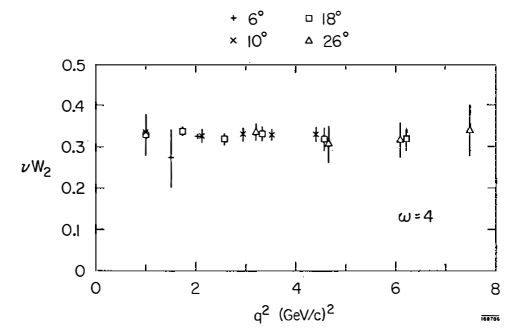
\includegraphics[width=0.75\textwidth]{./scattering/fig/no_q2_dep.png}
	\caption{Proton data showing no $Q^2$ dependence of $\nu W_2=F_2$ in the DIS region \cite{FriedmanKendall}.}
	\label{fig:noQ2F2}
\end{center}
\end{figure}

\section{Nuclear Structure Functions}
%TO DO:
% - Use something other than x for integral defining structure functions. Using multiple x's is confusing.

Having shown that the nucleons consist of structureless partons, we can define physics quantities in terms of the Quark-Parton Model (QPM). The QPM defines kinematic properties of the quarks and the nucleon structure functions in terms of constituent quark properties in the Bjorken limit. In this regime, Bjorken $x$ is the fraction of the momentum and energy contained by the parton scattered off of. To access the kinematics of the parton, we simply multiply the energy, momentum, and mass of the nucleon by $x$.

To analyze the structure functions of the nucleon, we first look at elastic scattering off of a parton. In this setup, we imagine that we have the means to determine what parton type the electron was scattered from. This is the same equation as Equation \ref{xs_no_struct}, but with $\alpha$ multiplied by the charge of the parton being scattered from, $e_i$, and replacing $M$ with $xM$ for the mass of the parton.

\begin{equation}
	\frac{d^2\sigma}{d\Omega dE^\prime} = \frac{\alpha^{2}e_{i}^{2}}{4E^{2}\sin^{4}\frac{\theta}{2}} \left[\cos^{2}\frac{\theta}{2} + \frac{Q^2}{2x^2M^2}\sin^{2}\frac{\theta}{2}\right] \delta\left(\nu-\frac{Q^2}{2xM}\right)
\end{equation}

Comparing this with the nuclear inelastic cross section, it is clear that the nuclear structure functions can be written in terms of parton structure functions. The parton structure functions can be derived using the same method as the nuclear structure functions.

\begin{subequations}
\begin{align}
	W_1^i = \frac{e_{i}^{2}Q^2}{4M^{2}x^{2}\nu}\delta\left(1-\frac{Q^2}{2Mx\nu}\right) \\
	W_2^i = \frac{e_{i}^{2}}{\nu}\delta\left(1-\frac{Q^2}{2Mx\nu}\right)
\end{align}
\end{subequations}

Defining $f_{i}\left(x\right)$ as the probability that a parton $i$ has the momentum fraction $x$, or parton distribution, we can then write the nucleon structure functions in terms of the parton structure functions. The delta function makes the integrals trivial.

\begin{subequations}
\begin{align}
	W_{1}\left(Q^{2},\nu\right) = \sum_{i}\int_0^1 \frac{e_{i}^{2}Q^2}{4M^{2}x^{2}\nu}f_{i}\left(x\right)\delta\left(1-\frac{Q^2}{2Mx\nu}\right) dx = \sum_{i} \frac{e_{i}^{2}}{2M}f_{i}\left(x\right) \\
	W_{2}\left(Q^{2},\nu\right) = \sum_{i}\int_0^1 \frac{e_{i}^{2}}{\nu}f_{i}\left(x\right)\delta\left(1-\frac{Q^2}{2Mx\nu}\right) dx = \sum_{i} \frac{e_{i}^{2}}{\nu}f_{i}\left(x\right)
\end{align}
\end{subequations}

Using the definitions of the $F$ structure functions in the previous sections, this formalism allows us to write them in terms of parton quantities.
\begin{subequations}
\begin{align}
	MW_1\left(Q^2,\nu\right) = \sum_i \frac{e_i^2}{2} f_i\left(x\right) \equiv F_1\left(x\right) \\
	\nu W_2\left(Q^2,\nu\right) = \sum_i e_i^2 x f_i\left(x\right) \equiv F_2\left(x\right)
\end{align}
\end{subequations}
These equations lead to a relation between the structure functions (in the Bjorken limit) called the Callan-Gross relation:
\begin{equation}
	F_2\left(x\right) = 2xF_1\left(x\right)
\end{equation}

%Utilizing this relation we can write the DIS cross section as:

Deriving the structure functions in terms of parton quantities also allows us to place constraints on the ratio of $F_2$ for the nucleons. Due to mass constraints, we can restrict this analysis to up ($q=2/3$), down ($q=-1/3$), and strange ($q=-1/3$) quarks. Since the proton and neutron, along with the up and down quarks, form an isospin doublet, we can relate their quark distributions and extend this to their antiquark distributions:

\begin{subequations}
\begin{align}
	u^p\left(x\right) = d^n\left(x\right) \equiv u \\
	d^p\left(x\right) = u^n\left(x\right) \equiv d \\
	s^p\left(x\right) = s^n\left(x\right) \equiv s 
\end{align}
\end{subequations}

Using these relations, we can write the nucleon structure functions and their ratio as:

\begin{subequations}
\begin{align}
	F_2^p = x\left[\frac{4}{9}\left(u+\bar{u}\right) + \frac{1}{9}\left(d+\bar{d}\right) + \frac{1}{9}\left(s+\bar{s}\right)\right] \\
	F_2^n = x\left[\frac{4}{9}\left(d+\bar{d}\right) + \frac{1}{9}\left(u+\bar{u}\right) + \frac{1}{9}\left(s+\bar{s}\right)\right]
\end{align}
\end{subequations}

\begin{equation}
	\frac{F_2^n}{F_2^p} = \frac{\left[\left(u+\bar{u}\right) + \left(s+\bar{s}\right)\right] + 4\left(d+\bar{d}\right)}{\left[\left(d+\bar{d}\right) + \left(s+\bar{s}\right)\right] + 4\left(u+\bar{u}\right)}
\end{equation}

This equation can be evaluated noting that by definition quark distributions must be positive. This naturally leads to a constraint on $F_2^n/F_2^p$ known as the Nachtmann inequality:

\begin{equation}
	\frac{1}{4} \leq \frac{F_2^n}{F_2^p} \leq 4
\end{equation}

%\textbf{INSERT PLOT FROM TALKS SHOWING NACHTMANN INEQUALITY IS SATISFIED}

%"These two form factors, $F_{1,2}(q^2)$, parametrize our ignorance of the detailed structure of the proton". \cite{HaM}
%
%\textbf{TALK MORE ABOUT THIS RELATION}
%
%The following relation allows the cross section to be written in terms of $F_2$ only.
%
%\begin{equation}
%	F_1 = \frac{F_2\left(1+Q^2/\nu^2\right)}{2x\left(1+R\right)}
%\end{equation}
%
%Here $x$ is the bjorken scaling variable and $R$ is the ratio of the longitudinal cross section to the transverse cross section, $\sigma_L/\sigma_T$.
%
%Plugging this in we arrive at
%
%\begin{equation}
%	\frac{d^2\sigma}{d\Omega dE^\prime}\left(E,E^\prime,\theta\right) = \frac{4\alpha^2\left(E^\prime\right)}{Q^4}\cos^2\left(\frac{\theta}{2}\right)F_2\left[\frac{1}{\nu}+\frac{\left(1+Q^2/\nu^2\right)}{xM\left(1+R\right)}\tan^2\left(\frac{\theta}{2}\right)\right]
%\end{equation}

\section{$R=\sigma_L/\sigma_T$}
If we instead approach DIS as the production and absorption of a virtual photon by a parton, we can extract a different structure function $R=\sigma_L/\sigma_T$, referred to as photonuclear R. That is, the ratio of the cross sections for absorbing longitudinal photons, $\sigma_L$, to transverse photons, $\sigma_T$. In the Bjorken limit, as in the previous section, $R\rightarrow 0$. In practice, the Bjorken limit is an imperfect approximation and it is useful to consider the effects of large, but finite, $Q^2$ and $\nu$.

We can write the DIS cross section in terms of these cross sections as
\begin{equation}
	\frac{d^2\sigma}{d\Omega dE^\prime}\left(E,E^\prime,\theta\right) = \Gamma\left[\sigma_T\left(x,Q^2\right)+\epsilon\sigma_L\left(x,Q^2\right)\right].
\end{equation}
In this equation, $\Gamma$ is the flux of transverse virtual photons and $\epsilon$ is the relative flux of longitudinal virtual photons. These are defined by
\begin{equation}
	\Gamma = \frac{\alpha KE^\prime}{2\pi^2Q^2E_0\left(1-\epsilon\right)}
\end{equation}
and
\begin{equation}
	\epsilon = \frac{1}{1+2\left(1+\nu^2/Q^2\right)\tan^2\left(\frac{\theta}{2}\right)}.
\end{equation}
Here, $K$ is the laboratory photon energy,
\begin{equation}
	K = \frac{W^2-M^2}{2M}.
\end{equation}

By comparing these equations to Equation \ref{eqn:x_dis_xs}, $F_1$ and $F_2$ can be related to $\sigma_L$, $\sigma_T$, and each other.

\begin{equation}
	\sigma_T = \frac{4\pi\alpha^2}{KM} F_1
\end{equation}

\begin{equation}
	\sigma_L = \frac{4\pi\alpha^2}{KM}\frac{1}{2x}\left[F_2 - 2xF_1\right]
\end{equation}

\begin{equation}
	F_1 = \frac{F_2\left(1+Q^2/\nu^2\right)}{2x\left(1+R\right)}
\end{equation}

Substituting this into our DIS cross section equation, we can eliminate $F_1$. This also makes it clear that we can easily access the $F_2$ structure functions by measuring cross section ratios.

\begin{equation}
	\frac{d^2\sigma}{d\Omega dE^\prime}\left(E,E^\prime,\theta\right) = \frac{4\alpha^2\left(E^\prime\right)}{Q^4}\cos^2\left(\frac{\theta}{2}\right)F_2\left[\frac{1}{\nu}+\frac{\left(1+Q^2/\nu^2\right)}{xM\left(1+R\right)}\tan^2\left(\frac{\theta}{2}\right)\right]
\end{equation}

If we measure the cross section ratios of two different targets at the same kinematics (that is the same $x$, $E$, $E^\prime$, and $\theta$), we find:

\begin{equation}
	\frac{\sigma_A}{\sigma_B} = \frac{F_2^A}{F_2^B} \frac{\left[\frac{1}{\nu}+\frac{\left(1+Q^2/\nu^2\right)}{xM\left(1+R^A\right)}\tan^2\left(\frac{\theta}{2}\right)\right]}{\left[\frac{1}{\nu}+\frac{\left(1+Q^2/\nu^2\right)}{xM\left(1+R^B\right)}\tan^2\left(\frac{\theta}{2}\right)\right]}
	\label{eqn:R_non_eq}
\end{equation}

As shown in Figure \ref{R_no_A}, historical data suggests that photonuclear R has no nuclear dependence to within $10\%$. If we assume that that there is no nuclear dependence, Equation \ref{eqn:R_non_eq} simplifies to:

\begin{figure}
\begin{center}
	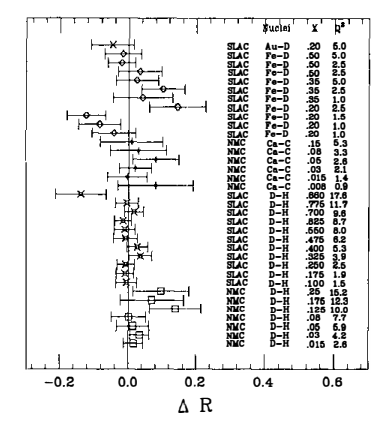
\includegraphics{./scattering/fig/R_LT.png}
	\caption{Historical data of $R=\sigma_L/\sigma_T$. This data shows measurements of the difference in $R$ between two nuclei. The data is consistent with no nuclear dependence \cite{GST}.}
	\label{R_no_A}
\end{center}
\end{figure}

\begin{equation}
	\frac{\sigma_A}{\sigma_B} = \frac{F_2^A}{F_2^B}
\end{equation}

By measuring the cross section ratios of targets in the DIS region, we can easily access the nuclear structure functions of the targets.

\section{$F_2^n/F_2^p$}
\label{sec:F2ratio}
The structure functions of the nucleons are common inputs to models. Making use of a Hydrogen target, the $F_2^p$ structure function is easily accessible. Unfortunately, there is no free neutron target. This absence means that there is no direct way to measure $F_2^n$. However, with the proper input, we can extract the ratio $F_2^n/F_2^p$.

To extract this ratio, we first define ``EMC-type'' ratios. These are simply the ratio of the nuclear structure function to the sum of the structure functions of its constituent nucleons. The ``EMC-type'' ratios for $^3$He and $^2$H are:

\begin{equation}
	R_{\text{EMC}}\left(^3\text{He}\right) = \frac{F_2^{^3\text{He}}}{2F_2^p + F_2^n}
\end{equation}

\begin{equation}
	R_{\text{EMC}}\left(^2\text{H}\right) = \frac{F_2^{^2\text{H}}}{F_2^p + F_2^n}
\end{equation}

These can be used to create a ``Super-Ratio'', $\mathcal{R}$, as the ratio of ``EMC-type'' ratios.

\begin{equation}
	\mathcal{R} = \frac{R_{\text{EMC}}\left(^3\text{He}\right)}{R_{\text{EMC}}\left(^2\text{H}\right)} = \frac{F_2^{^3\text{He}}}{2F_2^p + F_2^n} \cdot \frac{F_2^p + F_2^n}{F_2^{^2\text{H}}}
	\label{eqn:superR}
\end{equation}

Solving Equation \ref{eqn:superR} for $F_2^n/F_2^p$ makes it clear that the quantity can be easily extracted with a cross section ratio measurement and a model input for $\mathcal{R}$.

\begin{equation}
	\frac{F_2^n}{F_2^p} = \frac{F_2^{^3\text{He}}/F_2^{^2\text{H}} - 2\mathcal{R}}{\mathcal{R} - F_2^{^3\text{He}}/F_2^{^2\text{H}}}
\end{equation}

%\section{EMC Ratios}
%\textbf{Looking at the EMC-type ratios for Helium-3 and Tritium make it clear that we can extract the nucleon structure function ratio from the nuclear structure function ratio. We will use a calculation of the super ratio to do this extraction.}

%\subsection{First subsection}
%
%This is the first subsection of the first section of the first Chapter....
%
%
%\begin{table}[ht]
%\caption{Quarks, Leptons and Gauge Bosons}			% title of Table
%\centering										% used for centering table
%\begin{tabular}{l c c c r}							% centered columns (5 columns)
%\hline										%inserts single horizontal line
%Generation		& Quark 						& Electric Charge($\left | q_{e} \right |$)	& Mass($MeV/c^{2}$)	& Spin\\ 	 	% inserts table
%\hline										% inserts single horizontal line
%First				&Up (u)						& +2/3							& 1.7-3.1				& 1/2\\	%insertingbodyofthetable
%				& Down (d)					& -1/3							& 4.1-5.7				& 1/2\\[1ex]
%Second			& Charm (c)					& +2/3							& 1180-1340			& 1/2 \\
%				& Strange (s)					& -1/3 							& 80-130				& 1/2 \\[1ex]
%Third				& Top (t)						& +2/3 							& 172900$\pm$1500	& 1/2 \\
%				& Bottom (b) 					& -1/3		 					& 4130-4370			& 1/2 \\ [1ex]% [1ex] adds vertical space 
%\hline
%Generation		& Lepton						& Electric Charge($\left | q_{e} \right |$)	& Mass($MeV/c^{2}$)	& Spin\\ 
%\hline
%First				& Electron (e)					& -1								& 0.511				& 1/2\\
%				& Electron Neutrino ($\nu_{e}$)	& 0								& 0					& 1/2\\[1ex]
%Second			& Muon ($\mu$)				& -1								& 105.66				& 1/2\\
%				& Muon Neutrino ($\nu_{\mu}$)	& 0								& 0					& 1/2\\[1ex]
%Third				& Tau ($\tau$)					& -1								& 1776.84				& 1/2\\
%				& Tau Neutrino ($\nu_{\tau}$)		& 0								& 0					& 1/2\\[1ex]
%\end{tabular}
%\begin{tabular}{c c c c c}
%\hline
%Force			& Gauge Boson				& Electric Charge($\left | q_{e} \right |$)	& Mass($GeV/c^{2}$)	& Spin\\ 
%\hline
%Electromagnetic	& $\gamma$ (Photon)			& 0								& 0					& 1\\[1ex]
%Weak Nuclear		& $W^{\pm}$					& $\pm 1$							& 80.3980$\pm$0.025	& 1\\
%				& $Z^{0}$						& 0								& 91.1876$\pm$0.0021	& 1\\[1ex]
%Strong Nuclear		& g (8 Gluons)					& 0								& 0					& 1\\[1ex]
%\hline
%\end{tabular}
%\label{table:nonlin}								% is used to refer this table in the text
%\end{table}
%
%\newpage 
%
%
%\subsection{Second subsection}
%
%This is the second subsection....
%
%Here comes a Figure......
%
% \begin{figure}[!htbp]
%  \begin{center}
%    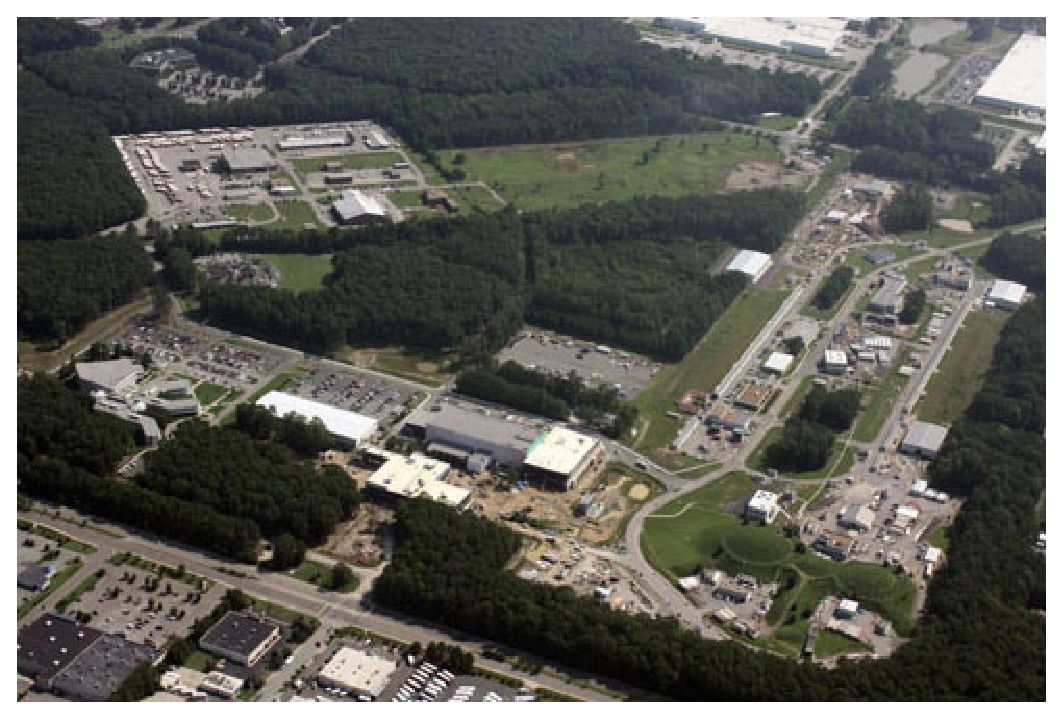
\includegraphics[angle=0, scale=0.85]{./chap1-intro/fig/Visit-JLab3.eps}
%  \end{center}
%  \caption[Aerial view of Jefferson Laboratory, Newport News, Virginia.]{
%    \footnotesize Aerial view of JLab
%  }
%  \label{fig:AerJLab}
%\end{figure}
%
%
%
%Use the label name to refer to  Figure  ~\ref{fig:AerJLab}.
%
%\subsubsection{Sub sub section a}
%
%This is a subsubsection
%
%\subsubsection {Sub sub section b}
%
%Another subsubsection......

